% figures/decision-tree.tex
% Standalone TikZ: two-branch decision tree comparing Target CPA bids (ch.02).
\documentclass[tikz,border=4pt]{standalone}
\usepackage{tikz}
\usetikzlibrary{arrows.meta,positioning,calc}

\definecolor{vcblue}{HTML}{1A5276}
\definecolor{vcteal}{HTML}{0E6655}
\definecolor{vcgray}{HTML}{555555}

\begin{document}
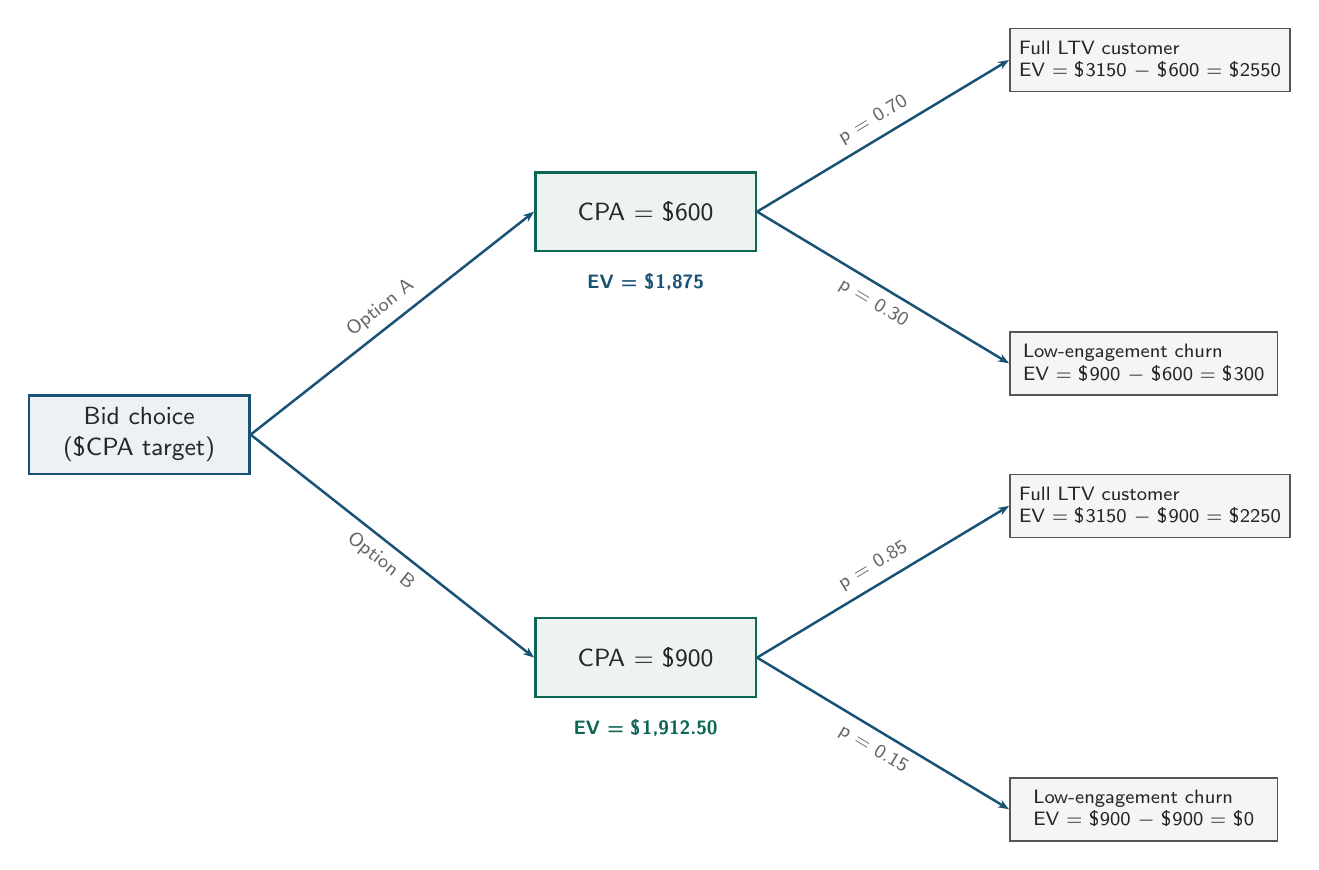
\begin{tikzpicture}[
  node distance=10mm,
  decision/.style={draw=vcblue, line width=0.9pt, fill=vcblue!8,
                   font=\sffamily\small, align=center,
                   minimum width=28mm, minimum height=10mm, text=black!85},
  chance/.style={draw=vcteal, line width=0.9pt, fill=vcteal!8,
                 font=\sffamily\small, align=center,
                 minimum width=28mm, minimum height=10mm, text=black!85},
  outcome/.style={draw=vcgray, line width=0.6pt, fill=vcgray!6,
                  font=\sffamily\scriptsize, align=left,
                  minimum width=34mm, minimum height=8mm, text=black!85},
  edge/.style={-{Stealth[length=4pt]}, vcblue, line width=0.9pt},
  label/.style={font=\sffamily\scriptsize, text=black!60},
]

  %% Root decision node
  \node[decision] (root) {Bid choice\\(\$CPA target)};

  %% Branch 1: CPA = $600
  \node[chance, above right=18mm and 36mm of root] (c600) {CPA = \$600};
  %% Branch 2: CPA = $900
  \node[chance, below right=18mm and 36mm of root] (c900) {CPA = \$900};

  %% Outcomes for CPA $600
  \node[outcome, above right=10mm and 32mm of c600] (o600h)
    {Full LTV customer\\EV = \$3150 $-$ \$600 = \$2550};
  \node[outcome, below right=10mm and 32mm of c600] (o600l)
    {Low-engagement churn\\EV = \$900 $-$ \$600 = \$300};

  %% Outcomes for CPA $900
  \node[outcome, above right=10mm and 32mm of c900] (o900h)
    {Full LTV customer\\EV = \$3150 $-$ \$900 = \$2250};
  \node[outcome, below right=10mm and 32mm of c900] (o900l)
    {Low-engagement churn\\EV = \$900 $-$ \$900 = \$0};

  %% Arrows root -> chance nodes
  \draw[edge] (root.east) -- node[label, above, sloped] {Option A} (c600.west);
  \draw[edge] (root.east) -- node[label, below, sloped] {Option B} (c900.west);

  %% Arrows chance -> outcomes (CPA $600)
  \draw[edge] (c600.east) -- node[label, above, sloped] {p = 0.70} (o600h.west);
  \draw[edge] (c600.east) -- node[label, below, sloped] {p = 0.30} (o600l.west);

  %% Arrows chance -> outcomes (CPA $900)
  \draw[edge] (c900.east) -- node[label, above, sloped] {p = 0.85} (o900h.west);
  \draw[edge] (c900.east) -- node[label, below, sloped] {p = 0.15} (o900l.west);

  %% EV rollback labels on chance nodes
  \node[font=\sffamily\scriptsize\bfseries, text=vcblue, below=1.5mm of c600]
    {EV = \$1,875};
  \node[font=\sffamily\scriptsize\bfseries, text=vcteal, below=1.5mm of c900]
    {EV = \$1,912.50};

\end{tikzpicture}
\end{document}
